\documentclass[11pt]{article}
\usepackage{color} %used for font color
\usepackage{amssymb} %maths
\usepackage{amsmath} %maths
\usepackage{bm}
\usepackage{epsfig}
\usepackage{soul}
\usepackage{subcaption}
\usepackage{listings}
\usepackage{authblk}
\usepackage{float}
\usepackage{graphicx}
\usepackage{multicol}
\usepackage{lipsum}
\topmargin-.5in
\textwidth6.6in
\textheight9in
\setlength{\columnsep}{0.6cm}
\oddsidemargin0in
\setlength\parindent{0pt}

%\def\fs{\scriptsize}
\usepackage{listings}
\usepackage{xcolor}

\DeclareMathOperator*{\E}{\mathbb{E}}

%New colors defined below
\definecolor{codegreen}{rgb}{0,0.6,0}
\definecolor{codegray}{rgb}{0.5,0.5,0.5}
\definecolor{codepurple}{rgb}{0.58,0,0.82}
\definecolor{backcolour}{rgb}{0.95,0.95,0.92}

%Code listing style named "mystyle"
\lstdefinestyle{mystyle}{
  backgroundcolor=\color{backcolour},   commentstyle=\color{codegreen},
  keywordstyle=\color{magenta},
  numberstyle=\tiny\color{codegray},
  stringstyle=\color{codepurple},
  basicstyle=\ttfamily\footnotesize,
  breakatwhitespace=false,         
  breaklines=true,                 
  captionpos=b,                    
  keepspaces=true,                 
  numbers=left,                    
  numbersep=5pt,                  
  showspaces=false,                
  showstringspaces=false,
  showtabs=false,                  
  tabsize=2
}

%"mystyle" code listing set
\lstset{style=mystyle}

\title{ \bf{Assignment V \\ MA797: Special Topics in Machine Learning}}
\author{Alp Tezbasaran$^{a}$}
\affil{\textit{$^{a}$Department of Nuclear Engineering NCSU, alptezbasaran@ncsu.edu}}
\date{December 13, 2019}
\begin{document}
\maketitle

\section{Recurrent Neural Network application of IMDB classification}

The task is to classify IMDB reviews as positive or negative. This task includes data which is in text format. The data is not only in text format but also constructed in sentences. The complete dataset includes 25000 movies reviews from IMBD, and labeled by sentiment (either positive or negative). Reviews are encoded into word index integers. For convenience, indexes are the ranks of frequency of each word. \medskip

Additionally, the dataset has 25000 out-of-sample testing set already separated. Before actualy training the model, data needs to be preprocessed, namely padded. The padding means the truncation of data longer than a specific limit and defining zero for shorter ones, basically used to make all the reviews the same length (500 words, vectors of 500 terms in this case).\medskip

Layer;
\begin{enumerate}
    \item Embedding layer
    \begin{itemize}
        \item Vector length = 16
    \end{itemize}
    \item LSTM layer
    \begin{itemize}
        \item 64 hidden states
    \end{itemize}
    \item Dense layer
    \begin{itemize}
        \item 1 output neuron (binary, 0 for bad or 1 for good sentiment)
        \item Sigmoid activation
    \end{itemize}
\end{enumerate}

Here architecture being the same, some modeling parameters are to be tuned. Vector length and number of hidden LSTM states can be considered as hyperparameters where first one is a measure of output shape of embedding layer and the second one defines the actual number of LSTM layers to be trained, respectively. Embedding can be considered as the transformation of one-hot represented vectors of words into a a continuous and dense latent space and number of layers is the number of LSTM layers to be trained and pipe lined. Since there is no optimized way to pick these values, predictive model is trained for all possible combinations and testing accuracy for out-of-sample data is evaluated.

Additional model details;
\begin{itemize}
    \item Optimizer: Adam
    \item Loss: Binary crossentropy
    \item Metric: Binary accuracy
    Validation split ratio: 0.2
    \item Minimum epocs: 10
\end{itemize}

The assignment specifies the number of epochs as 10 or more. However, the callback functions are used here where if there is no improvement for 10 epochs (patience), training is terminated and the best model is saved. Patience value of 10 ensures that there are at least 10 epoch, and for larger models, there will be more epochs if necessary. Maximum number of epochs are set as 50 but no parameter couple needed more than 15 epochs. The training and validation trends for each epoch es also saved with Tensorboard callbacks, which can be observed later if necessary.

\begin{figure}[H]
\centering
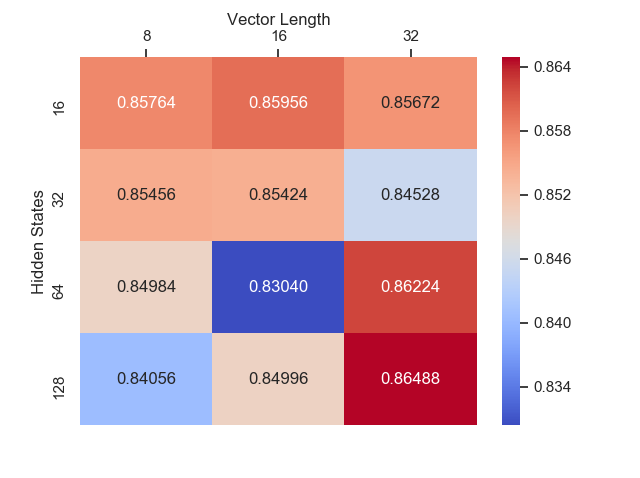
\includegraphics[width=0.65\columnwidth]{pics/rnn_hyper.png}
\captionsetup{justification=centering}
\caption{Out-of-sample testing accuracy for different vector and hidden LSTM state numbers}
\label{fig:q1_acc}
\end{figure}

From Figure \ref{fig:q1_acc}, it is obvious that there is no real gain from going short vector lengths and number of hidden LSTM states to longer vector representation and more hidden states. The highest accuracy is achieved when vector length is $\bm{32}$ and number of hidden states is $\bm{128}$ but, there is not an observable trend that suggests increasing these parameters is profitable in the sense of out-of-sample accuracy. This can be seen with the accuracy achieved for vector length of 16 and hidden states of 64. The out-of-sample accuracy for this combination is worst in all the parameter space investigated.\medskip

Furthermore, the maximum difference between the achieved accuracy values is less than 0.03 which is relatively small. So, observing a real trend between these parameters doesn't offer much for this problem and the architecture defined for this problem. \medskip

Overall out-of-sample testing accuracy achieved for is problem is around $\bm{0.85}$-$\bm{0.86}$ levels. 

The code for the fine-tuned model construction is shown in the listing below. Note that all information is saved including the model pickles for future use.

\begin{lstlisting}[language=Python, basicstyle=\tiny, caption=Python code for the fine-tuned LSTM model]
import tensorflow as tf
from tensorflow.keras.datasets import imdb
import pandas as pd
import shutil
import os

cwd = os.getcwd()
shutil.rmtree(cwd + '\\rnn_*',ignore_errors=True)

tf.__version__
# Set CPU as available physical device
my_devices = tf.config.experimental.list_physical_devices(device_type='CPU')
tf.config.experimental.set_visible_devices(devices= my_devices, device_type='CPU')
tf.random.set_seed(0)

# Data import parameters
number_of_words = 5000
max_len = 500

# Import data
(X_train, y_train), (X_test, y_test) = imdb.load_data(num_words = number_of_words)

# Padding all sequences to be the same lenght
X_train = tf.keras.preprocessing.sequence.pad_sequences(X_train, max_len)
X_test = tf.keras.preprocessing.sequence.pad_sequences(X_test, max_len)

# Define model architecture
def create_RNN_model(hidden_states = 64, vector_length = 16):
  # Create the model
  model = tf.keras.Sequential()
  # 1st Embedding layer
  model.add(tf.keras.layers.Embedding(input_dim = number_of_words, output_dim = vector_length, input_shape = (X_train.shape[1],)))
  # 1st LSTM layer
  model.add(tf.keras.layers.LSTM(units = hidden_states, activation = 'tanh'))
  # Output layer
  model.add(tf.keras.layers.Dense(units = 1, activation ='sigmoid'))
  # Compile
  model.compile(optimizer = 'adam', loss = 'binary_crossentropy', metrics=['binary_accuracy'])
  return(model)

# Iterate over parameters
vector_length = [8,16,32]
hidden_states = [16,32,64,128]

print('Training all')
metrics = []
for vl in vector_length:
  for hs in hidden_states:
    print('+'*50)
    print('vector length = ', vl, 'hidden states = ',hs)
    print('+'*50)
    # Tensorboard
    log_dir = 'rnn_log_hs'+ str(hs) + '_vec_len_' + str(vl)
    tensorboard_callback = tf.keras.callbacks.TensorBoard(log_dir=log_dir, update_freq='epoch', profile_batch = 0)
    # Early Stop
    early_stoppping = tf.keras.callbacks.EarlyStopping(patience=10, monitor='val_loss', verbose=1)
    # Save
    save_checkpoint = tf.keras.callbacks.ModelCheckpoint(filepath= 'rnn_log_hs'+ str(hs) + '_vec_len_' + str(vl) + '.h5',
                                                         save_best_only=True,
                                                         monitor='val_loss',
                                                         verbose=1)
    # Create Model
    model = create_RNN_model(vector_length = vl, hidden_states = hs)
    # Fit
    history = model.fit(X_train, y_train, epochs = 20,  validation_split = 0.2, use_multiprocessing = True,
                                                                   verbose = 1, callbacks = [tensorboard_callback, early_stoppping, save_checkpoint])
    # Metrics
    training_loss = history.history['loss'][-1]
    validation_loss = history.history['val_loss'][-1]
    training_accuracy = history.history['binary_accuracy'][-1]
    validation_accuracy = history.history['val_binary_accuracy'][-1]
    test_loss, test_accuracy = model.evaluate(X_test, y_test, verbose = 2)
    print('Test accuracy = ',test_accuracy)
    metrics.append({'hidden_state':hs,
                    'vector_length':vl,
                    'validation_accuracy':validation_accuracy,
                    'training_loss':training_loss,
                    'validation_loss':validation_loss,
                    'training_accuracy':training_accuracy,
                    'test_loss':test_loss,
                    'test_accuracy':test_accuracy
                    })
print('Training Over')
df = pd.DataFrame(metrics)
df.to_pickle('./rnn_metrics.pkl')
print('Database ready')
\end{lstlisting}

\newpage

\section{Decision Tree and Random Forest Classifiers}

Data for a classifier model is \textit{'Pima-Data-Adjusted.mat'} from UC Irvin Machine Learning Database, and distributions of each feature and labels are shown in Figure \ref{fig:q2_data}. Data basically tells if a person has diabetes or not based on 8 features.

\begin{figure}[H]
\centering
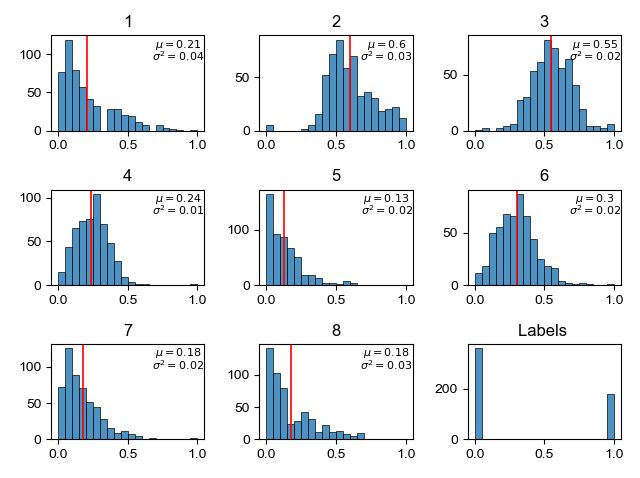
\includegraphics[width=0.85\columnwidth]{pics/data.png}
\captionsetup{justification=centering}
\caption{Distributions of features and labels}
\label{fig:q2_data}
\end{figure}

The data is preprocessed, adjusted from the database to remove entries with missing data, and these data have been normalized. So looking at the distribution has no informative value. The histograms are created to investigate if there are outliers or distributions are highly skewed. The data seems slightly imbalanced towards non-diabetes cases but overall distributions do not prevent a model construction. \medskip

The goal is to create a fine-tuned classifiers which use decision tree and random forest methods. For this reason python library SciKitLearn is employed for both classifiers and cross-validated fine tuning. \medskip

\subsection{Decision Tree Classifier}
Decision tree classifier is a 'supervised classifier' where data is continuosly split according to a certain parameter based on a metric which has following hyperparemeters for this study:
\begin{itemize}
    \item Depth of the decision tree
    \item Minimum node size
\end{itemize}

and the metric to be optimized is \emph{gain in error reduction}. First data is split into 70\% training and 30\% of testing portions. \medskip

To train a classifier scikitlearn's \emph{sklearn.tree.DecisionTreeClassifier} is defined. Additionally, to fine tune hyperparameters, \emph{GridSearchCV} class is imported from \emph{sklearn.model\_selection} module. This class is basically an exhaustive grid search method, which iterates all possible hyperparameter combinations in a brute force way. Following code snippet shows the classifier definition and fine tuning with k-fold cross validation capability. 

\begin{lstlisting}[language=Python, basicstyle=\tiny, caption=Python code snippet for fine tuning the \underline{Decision Tree } classifier]
# Decision Tree
# Fitting Decision Tree Classification to the Training set
from sklearn.tree import DecisionTreeClassifier
dt_classifier = DecisionTreeClassifier(random_state = 0)
# use a full grid over all parameters
param_grid = {"max_depth": [None, 50, 20, 11, 10, 9, 8, 7, 6, 5, 4, 3, 2],
              'min_samples_split': [40, 38, 37,  36, 35, 34, 33, 32, 31, 30, 20, 10, 9, 8]}

# run grid search
grid_search = GridSearchCV(dt_classifier, param_grid=param_grid, cv=5, n_jobs = -1, return_train_score=True)
start = time()
grid_search.fit(X, y)
print("GridSearchCV took %.2f seconds for %d candidate parameter settings."
      % (time() - start, len(grid_search.cv_results_['params'])))
print(grid_search.best_params_)
\end{lstlisting}

The snippet shows the definition of 5-fold cross validation during the tuning. The criterion for the classifier is defines as \emph{entropy} per instructors request. Following figure shows the accuracy obtained for each iteration, the hyperparameter couples. Iterative search is defined in a way tat it starts from the most complex model which evidently over fits to training data. The training and testing accuracy values are the mean values of 5-fold cross validation, meaning that the 5 accuracy values obtained for one hyperparameter couple are averaged.\medskip

\begin{figure}[H]
\centering
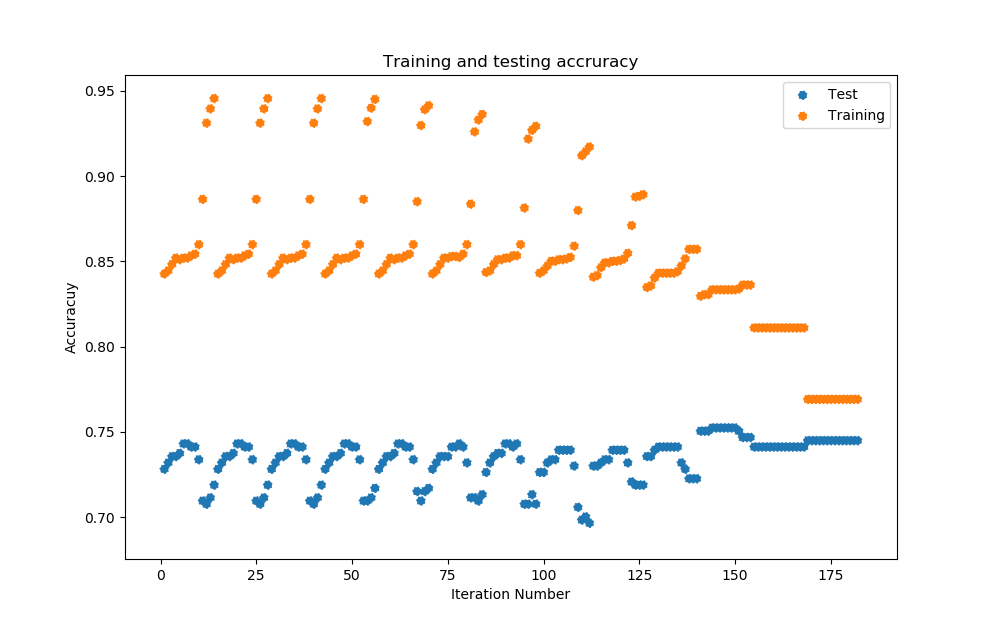
\includegraphics[width=0.85\columnwidth]{pics/q2_dt.png}
\captionsetup{justification=centering}
\caption{Distributions of features and labels}
\label{fig:q2_dt}
\end{figure}

In \ref{fig:q2_dt}, looking at the trend is meaningless, the recognizable patterns can be observed when one of the hyperparameters is kept constant and other one is iterated but the actual outcome is based on the parameters which yield minimum testing loss. In \emph{GridSearchCV} object the scoring is defined as the error to be minimized which ensures that the error is reduction is maximized, in other words gain in error reduction. After iterating over all the parameter pairs (182 combinations) shown in Listing for Decision Tree, following values for hyperparameters are obtained.
\begin{itemize}
    \item 'max\_depth': 4 
    \item 'min\_samples\_split': 36
\end{itemize}

and the out of sample testing accuracy for this pair is approximately, $\bm{0.747}$ which is comparable with the mean cross-validation in-sample testing accuracy of 0.711

\subsection{Random Forest Classifier}
After successful training a decision tree classifier, many of them ensembled to have a more representative model. This method is called random forest (another supervised method) which is basically training a lot of decision trees and making the decision based on the majority vote. \medskip

Like, decision trees, random forest classifiers also have hyperparameters. All hyperparameters and scoring methods of decision trees also apply to random forests and they are used to train individual decision trees. Additionally, number of trees can be defined. If there are a lot of trees the model is prone to over fit to training data. But truncating after a certain number of decision trees, can prevent this. There is no optimal number, for each dataset and model parameters. So, fine tuning must be employed to investigate the optimal number of trees. Decision tree hyperparameters values are the ones computed in the previous section.\medskip

The training is made by using the scikitlearn's, \emph{sklearn.ensemble.RandomForestClassifier} module. Aside the decision tree parameters, \emph{n\_estimators} defines the number of trees.\medskip

The same split data with decision tree classifier is used without shuffling to make sure we are training the model for the same data and testing with the same data to have a comperative idea between methods. \medskip

The same exhaustive brute-force search method is employed for this section, but there is only hyperparameter, \emph{n\_estimators} and similar to decision tree model construction. 5-fold cross validation strategy is adopted. 

\begin{lstlisting}[language=Python, basicstyle=\tiny, caption=Python code snippet for fine tuning the \underline{Random Forest} classifier]
# RF - Grid search with k-fold cross validation
num_trees = range(5,1000 + 1,5)
num_trees_2 = range(55,65,1)

# run grid search
def rf_search(num_trees):
  # use a full grid over all parameters
  param_grid = {"n_estimators": num_trees}
  grid_search = GridSearchCV(rf_classifier, param_grid=param_grid, cv=5, n_jobs = -1, return_train_score=True)
  start = time()
  grid_search.fit(X, y)
  print("GridSearchCV took %.2f seconds for %d candidate parameter settings." % (time() - start, len(grid_search.cv_results_['params'])))
  print(grid_search.best_params_)
  
  plt.figure()
  plt.scatter(num_trees, grid_search.cv_results_['mean_test_score'], linestyle  = 'dotted', label = 'Test')
  plt.scatter(num_trees, grid_search.cv_results_['mean_train_score'], linestyle  = 'dotted', label = 'Training')
  plt.title('Training and testing accruracy')
  plt.xlabel('Number of Trees')
  plt.ylabel('Accuracuy')
  plt.legend()
  
 
rf_search(num_trees_2)
  
rf_classifier = RandomForestClassifier(n_estimators = 59, max_depth = 4, min_samples_split = 36, random_state = 0)
rf_classifier.fit(X_train, y_train)
rf_classifier.fit(X_train, y_train)
# Predicting the Test set results
y_pred = rf_classifier.predict(X_test)
rf_score = rf_classifier.score(X_test, y_test)
# Making the Confusion Matrix
from sklearn.metrics import confusion_matrix
cm_rf = confusion_matrix(y_test, y_pred)
\end{lstlisting}

The fine tuning is done in two stages, first a space from 5 to 1000 increment by 5, is investigated to yield the best average in-sample test accuracy. Then the yielded value of interest as median search space is expanded to -5 to +5 of yielded value with increment of 1. Since number of trees must be an integer this strategy calculates the optimum number of trees. Figures \ref{fig:q2_rf1} and \ref{fig:q2_rf2} show the average testing and training scores (accuracy) as a function of number of estimators (trees).
\begin{multicols}{2} 

\begin{figure}[H]
\centering
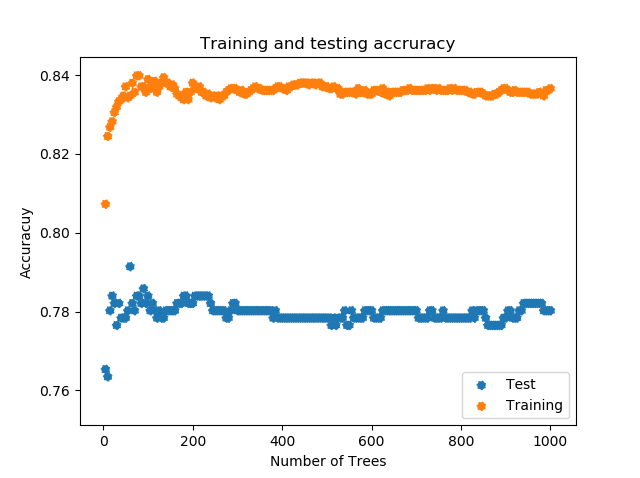
\includegraphics[width=0.98\columnwidth]{pics/q2_rf1.png}
\captionsetup{justification=centering}
\caption{Distributions of features and labels}
\label{fig:q2_rf1}
\end{figure}

\begin{figure}[H]
\centering
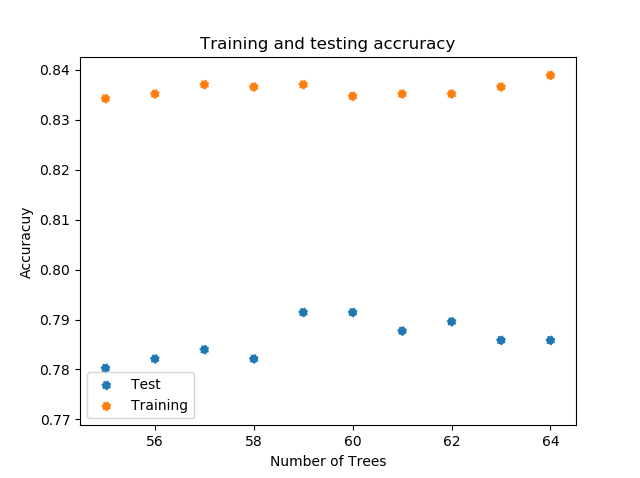
\includegraphics[width=0.98\columnwidth]{pics/q2_rf2.png}
\captionsetup{justification=centering}
\caption{Distributions of features and labels}
\label{fig:q2_rf2}
\end{figure}

\end{multicols}


As seen in Figure \ref{fig:q2_rf1} accuracy values of training data reaches and fluctuates around 0.84 and testing data plateaus after after 200 estimators.\medskip

The optimum number of trees is found to be $\bm{59}$. A model trained with 59 estimator, yields out-of sample testing accuracy of $\bm{0.79}$, a few percents higher than that of a single decision tree. \medskip

Following table and confusion matrices are the comparison between fine-tuned decision tree and random forest classifiers.

\bgroup
\def\arraystretch{1.5}%  1 is the default, change whatever you need
\begin{table}[H]
\centering
\caption{Obtained accuracies for different models}
\begin{tabular}{|l|c|c|}
\hline
 &\textbf{Decision Tree}   & \ \textbf{Random Forest}  \\ \hline
\textbf{Ave Training} & 0.946 & 0.839 \\ \hline
\textbf{Ave In-sample testing} & 0.752 & 0.791\\ \hline
\textbf{Out-of-sample testing} & 0.747 & 0.790 \\ \hline
\end{tabular}
\label{table:and}
\end{table}
\egroup

Confusion matrices:
$$
cm_{decision tree}=
 \begin{bmatrix}
 \begin{array}{rr}
90 &  15  \\
26 &  31 
\end{array}   
\end{bmatrix} \quad
cm_{random forest}=
 \begin{bmatrix}
 \begin{array}{rr}
97 &  8  \\
26 &  31 
\end{array}   
\end{bmatrix}
$$

The winner is fine-tuned Random Forest classifier with 0.79 out-of-sample accuracy value. This is expected because a lot of decision trees are ensembled to make decision rather than one. 

\end{document}
 